\begin{GreyBox}
    \vskip-1cm
    \begin{block}{\GHead{Results}}

        \begin{center}
            \vskip-2.0cm
            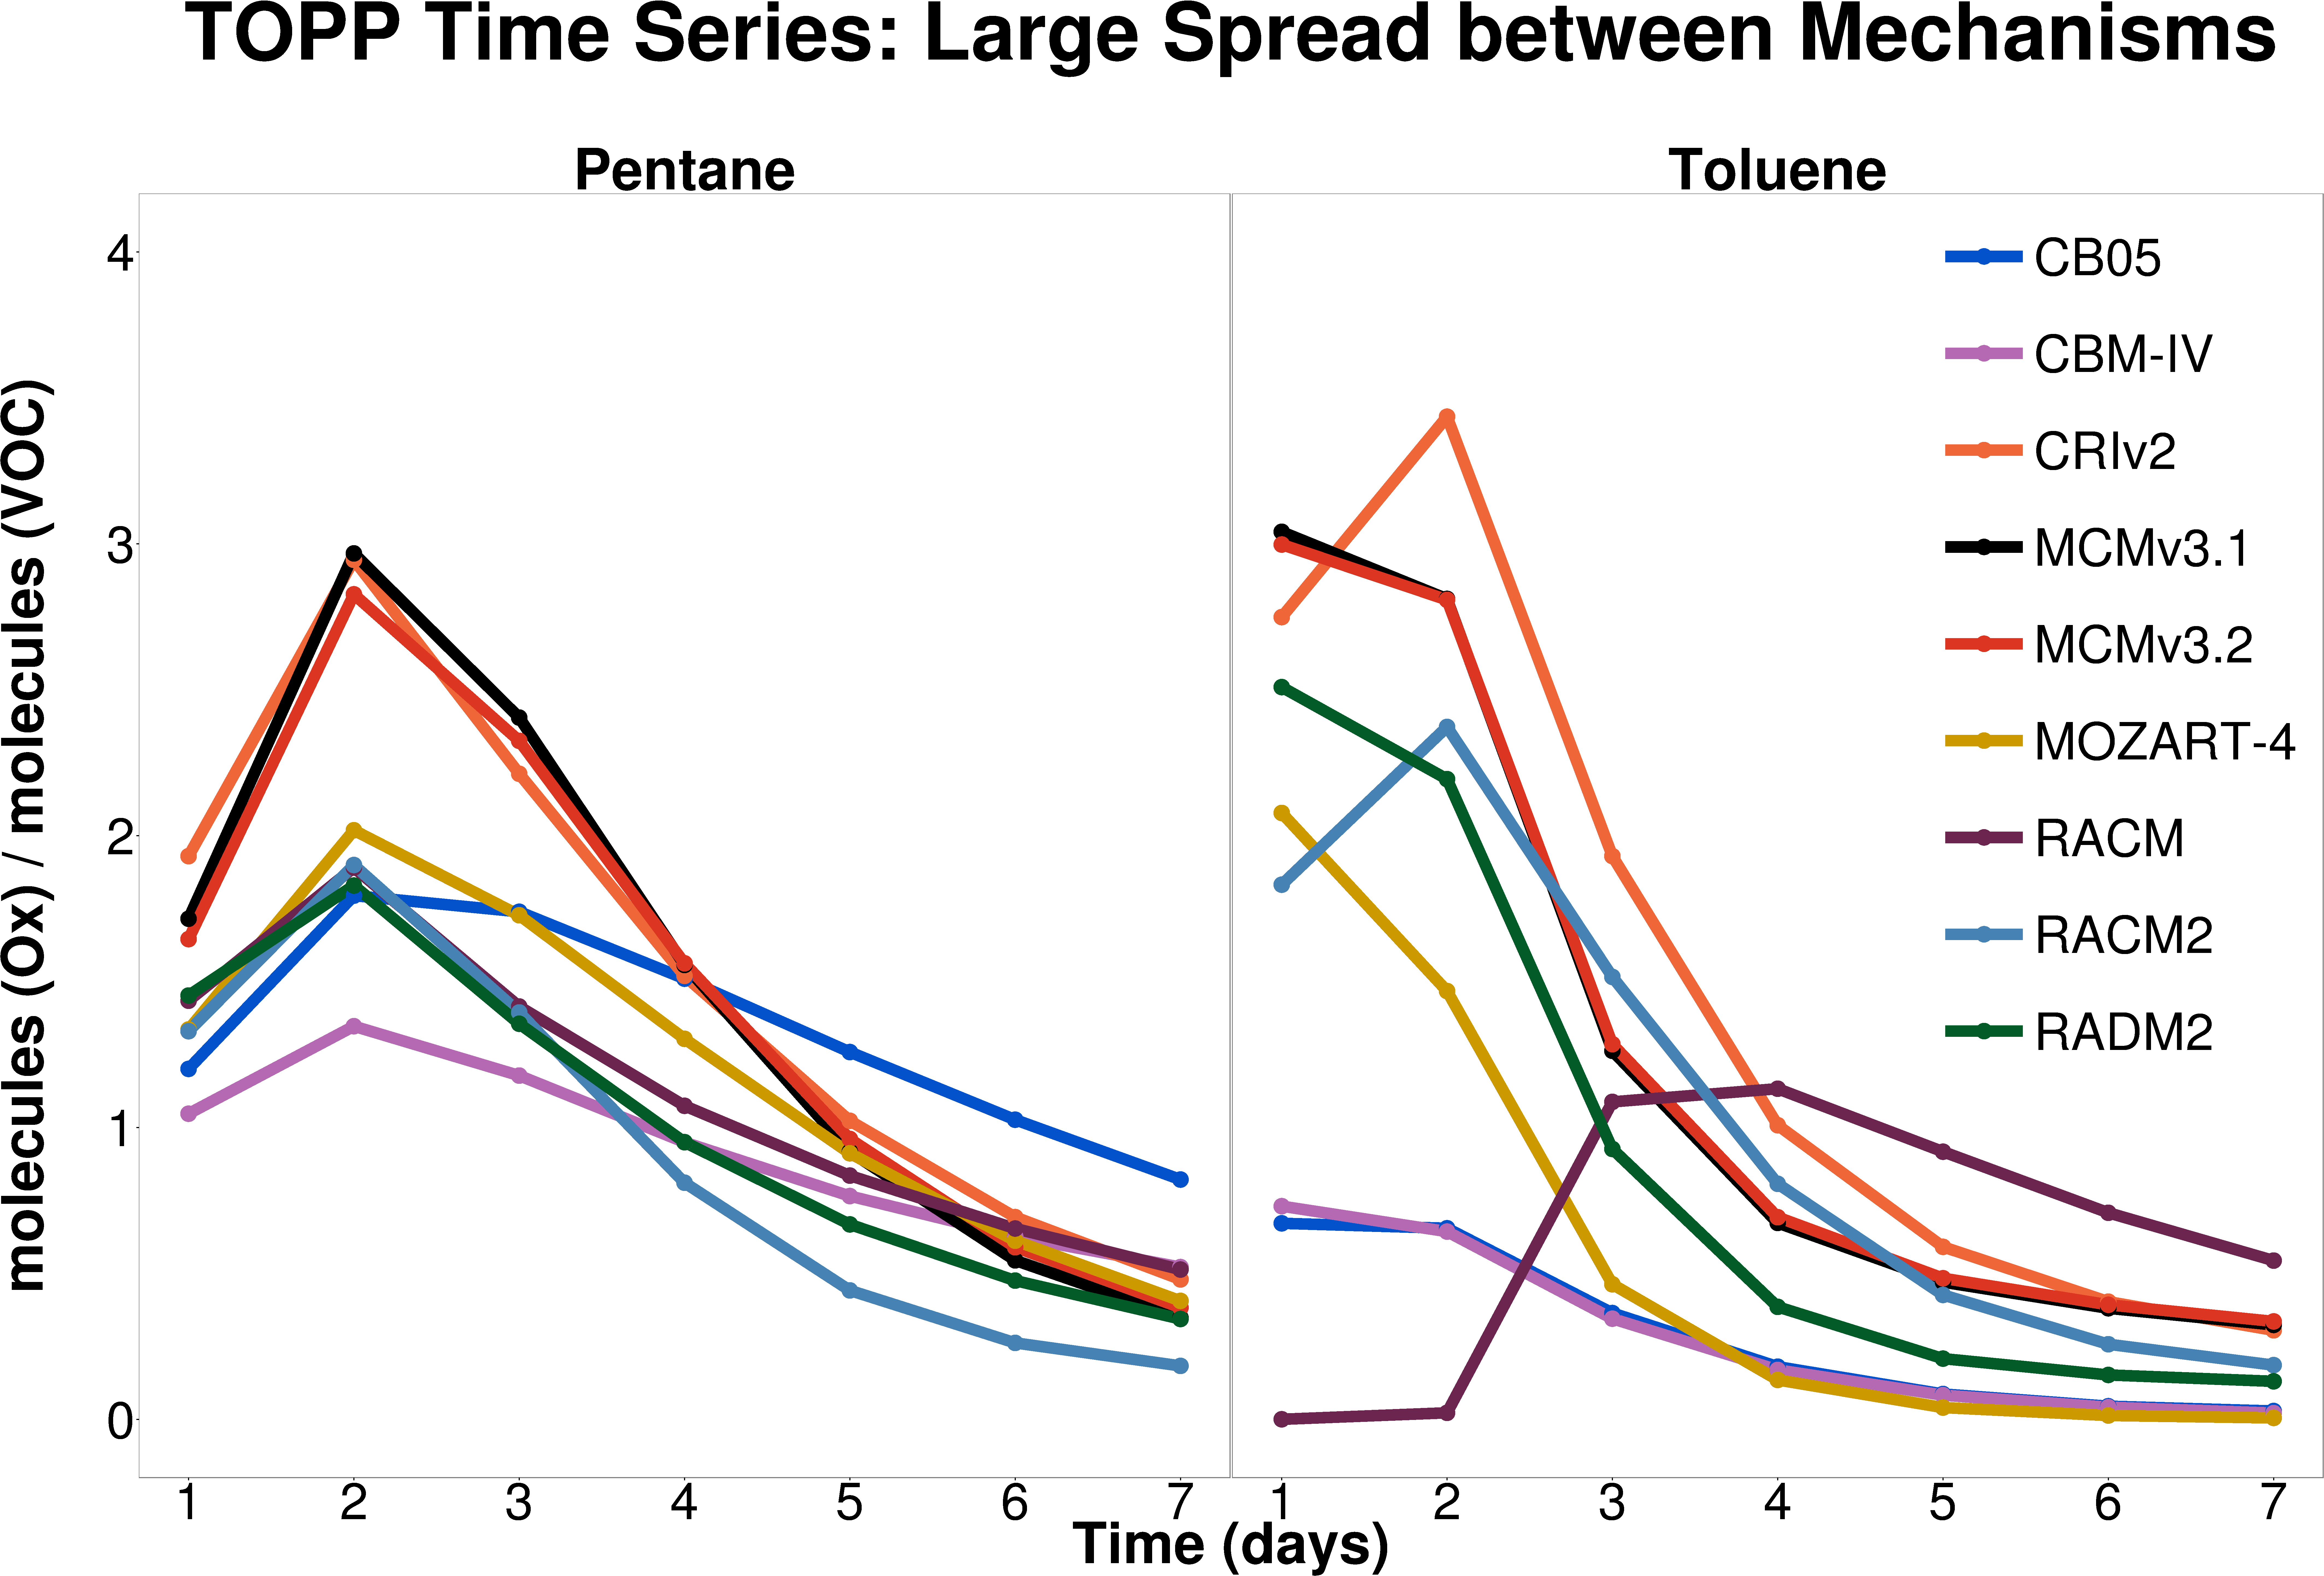
\includegraphics[scale=0.2]{img/TOPPs}
        \end{center}
        \begin{columns}[c]
            \column{.5\textwidth}
                \begin{center}
                    \includegraphics[scale=0.145]{img/carbon_percent_total_Ox_production}
                \end{center}
            \column{.5\textwidth}
                \begin{center} 
                    \vskip-1cm
                    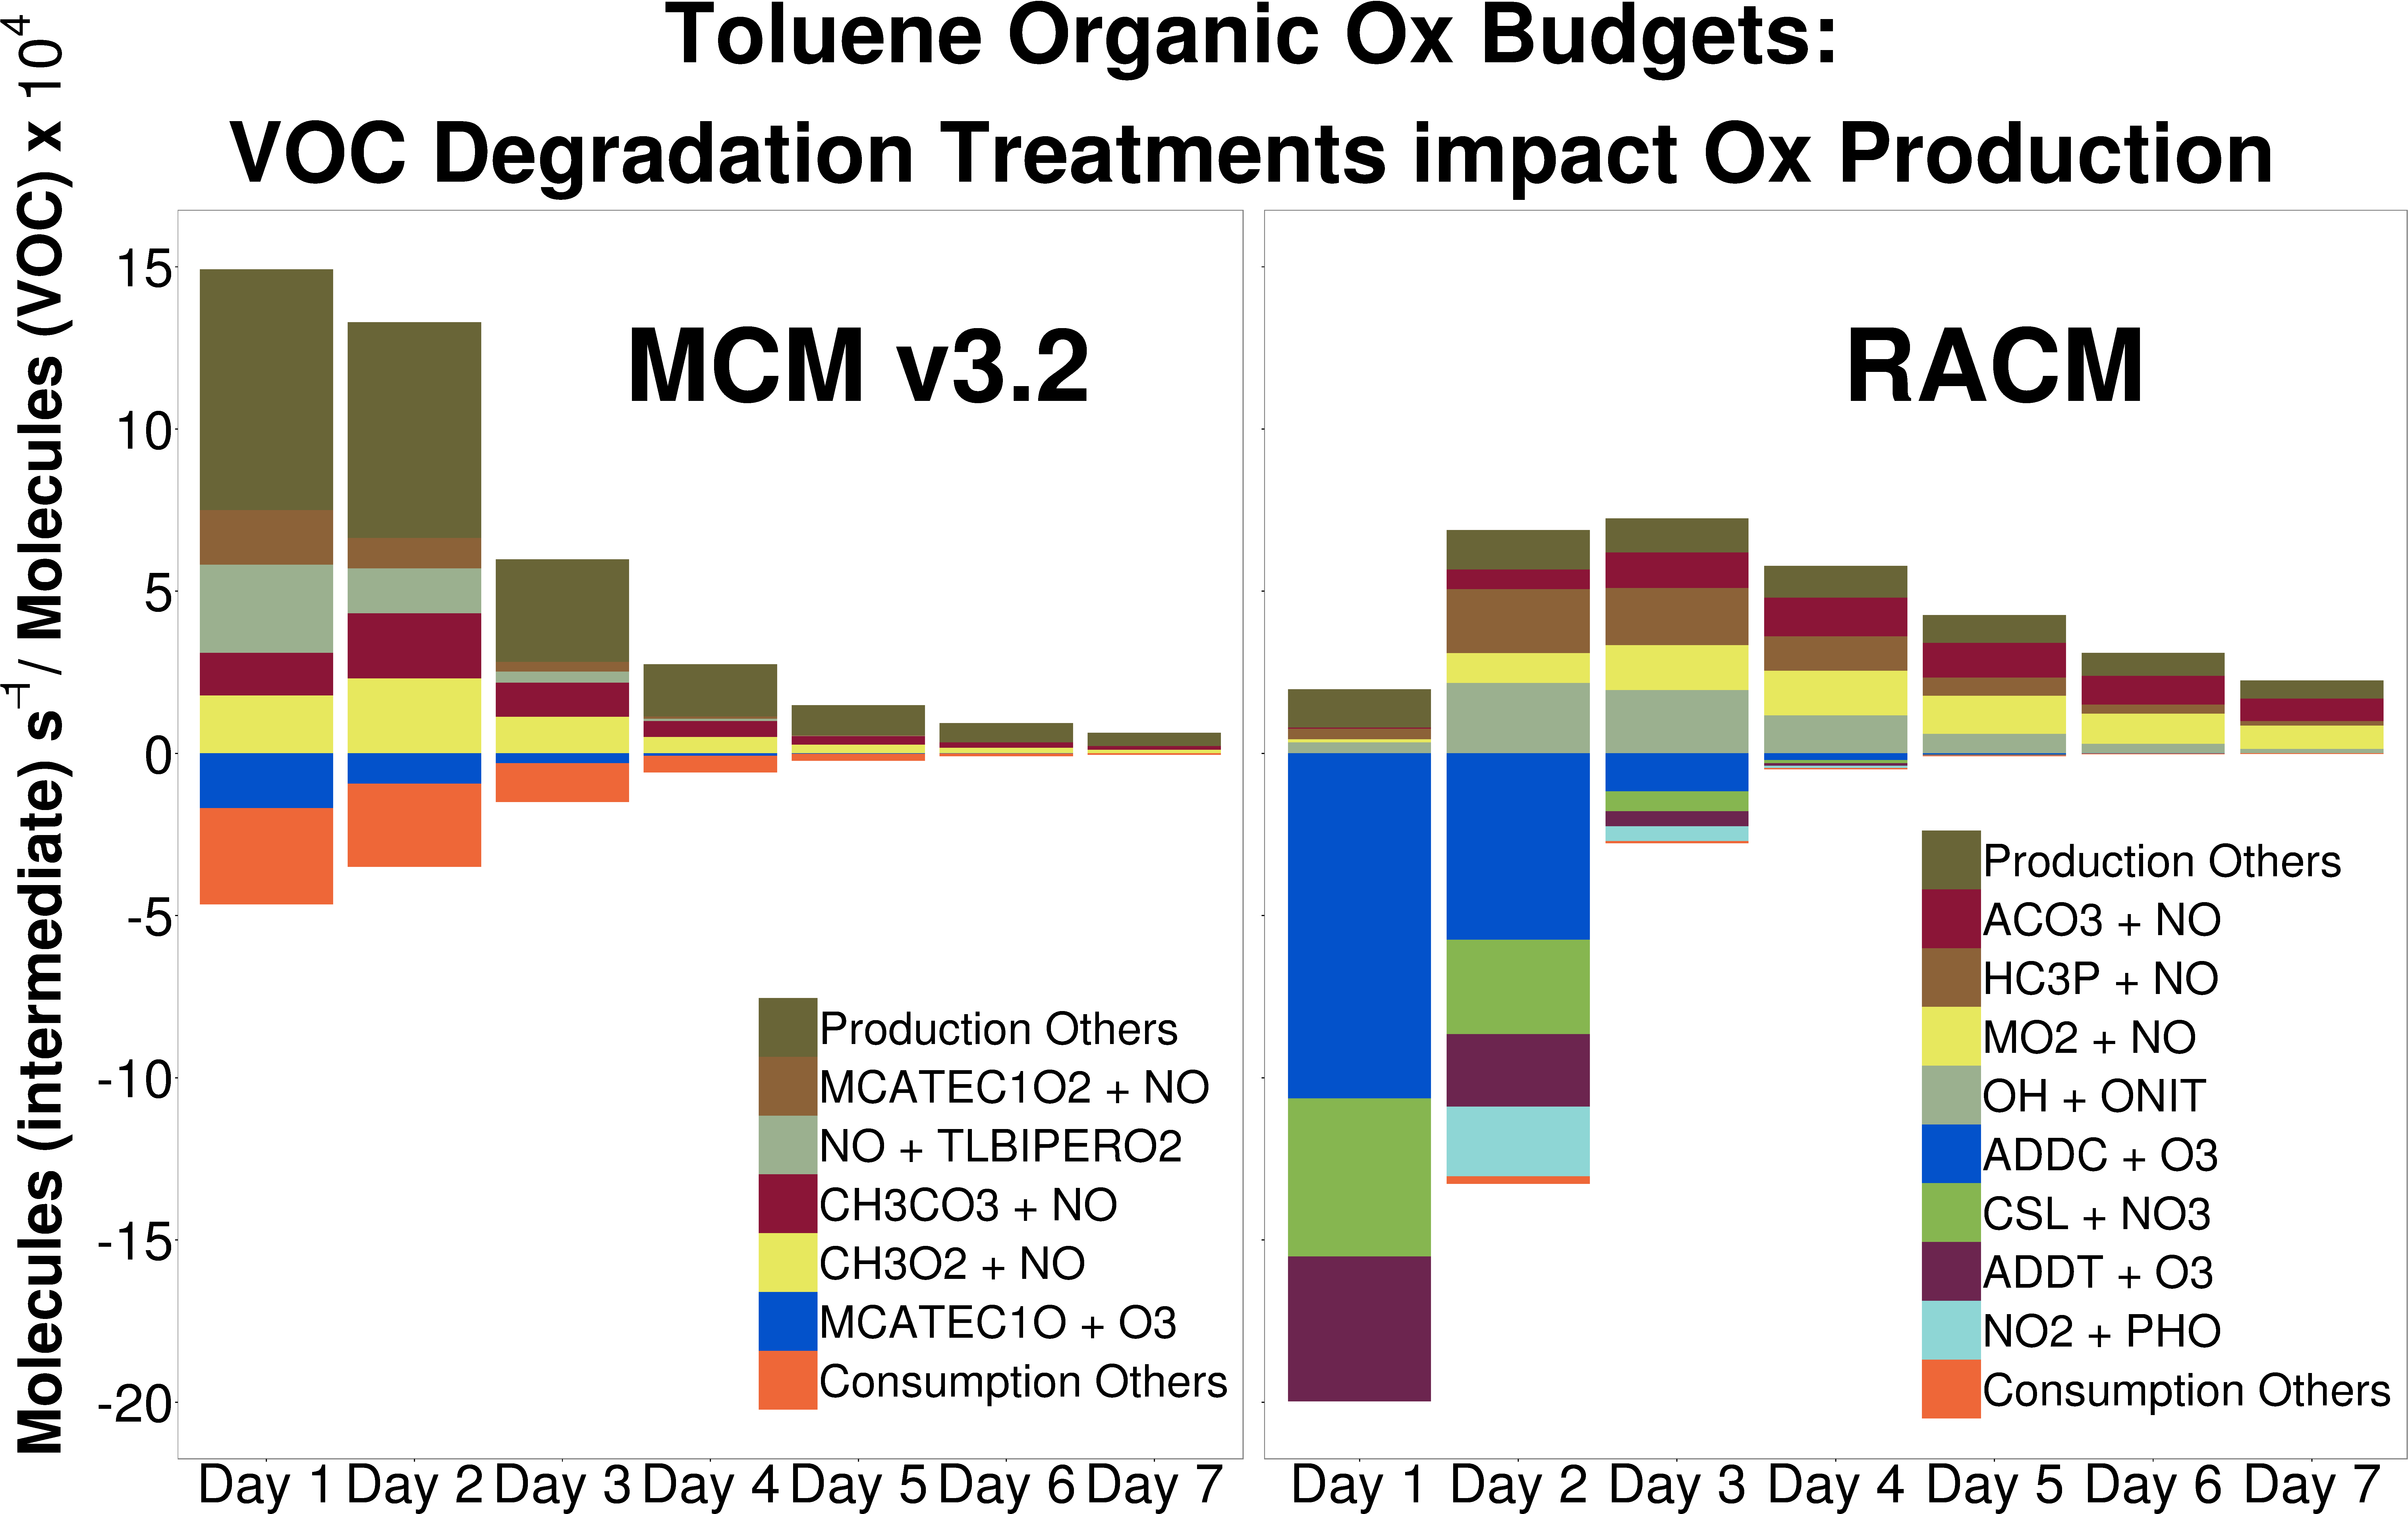
\includegraphics[scale=0.14]{img/TOL_MCM_RACM_Ox_intermediates} 
                    \vskip4cm
                    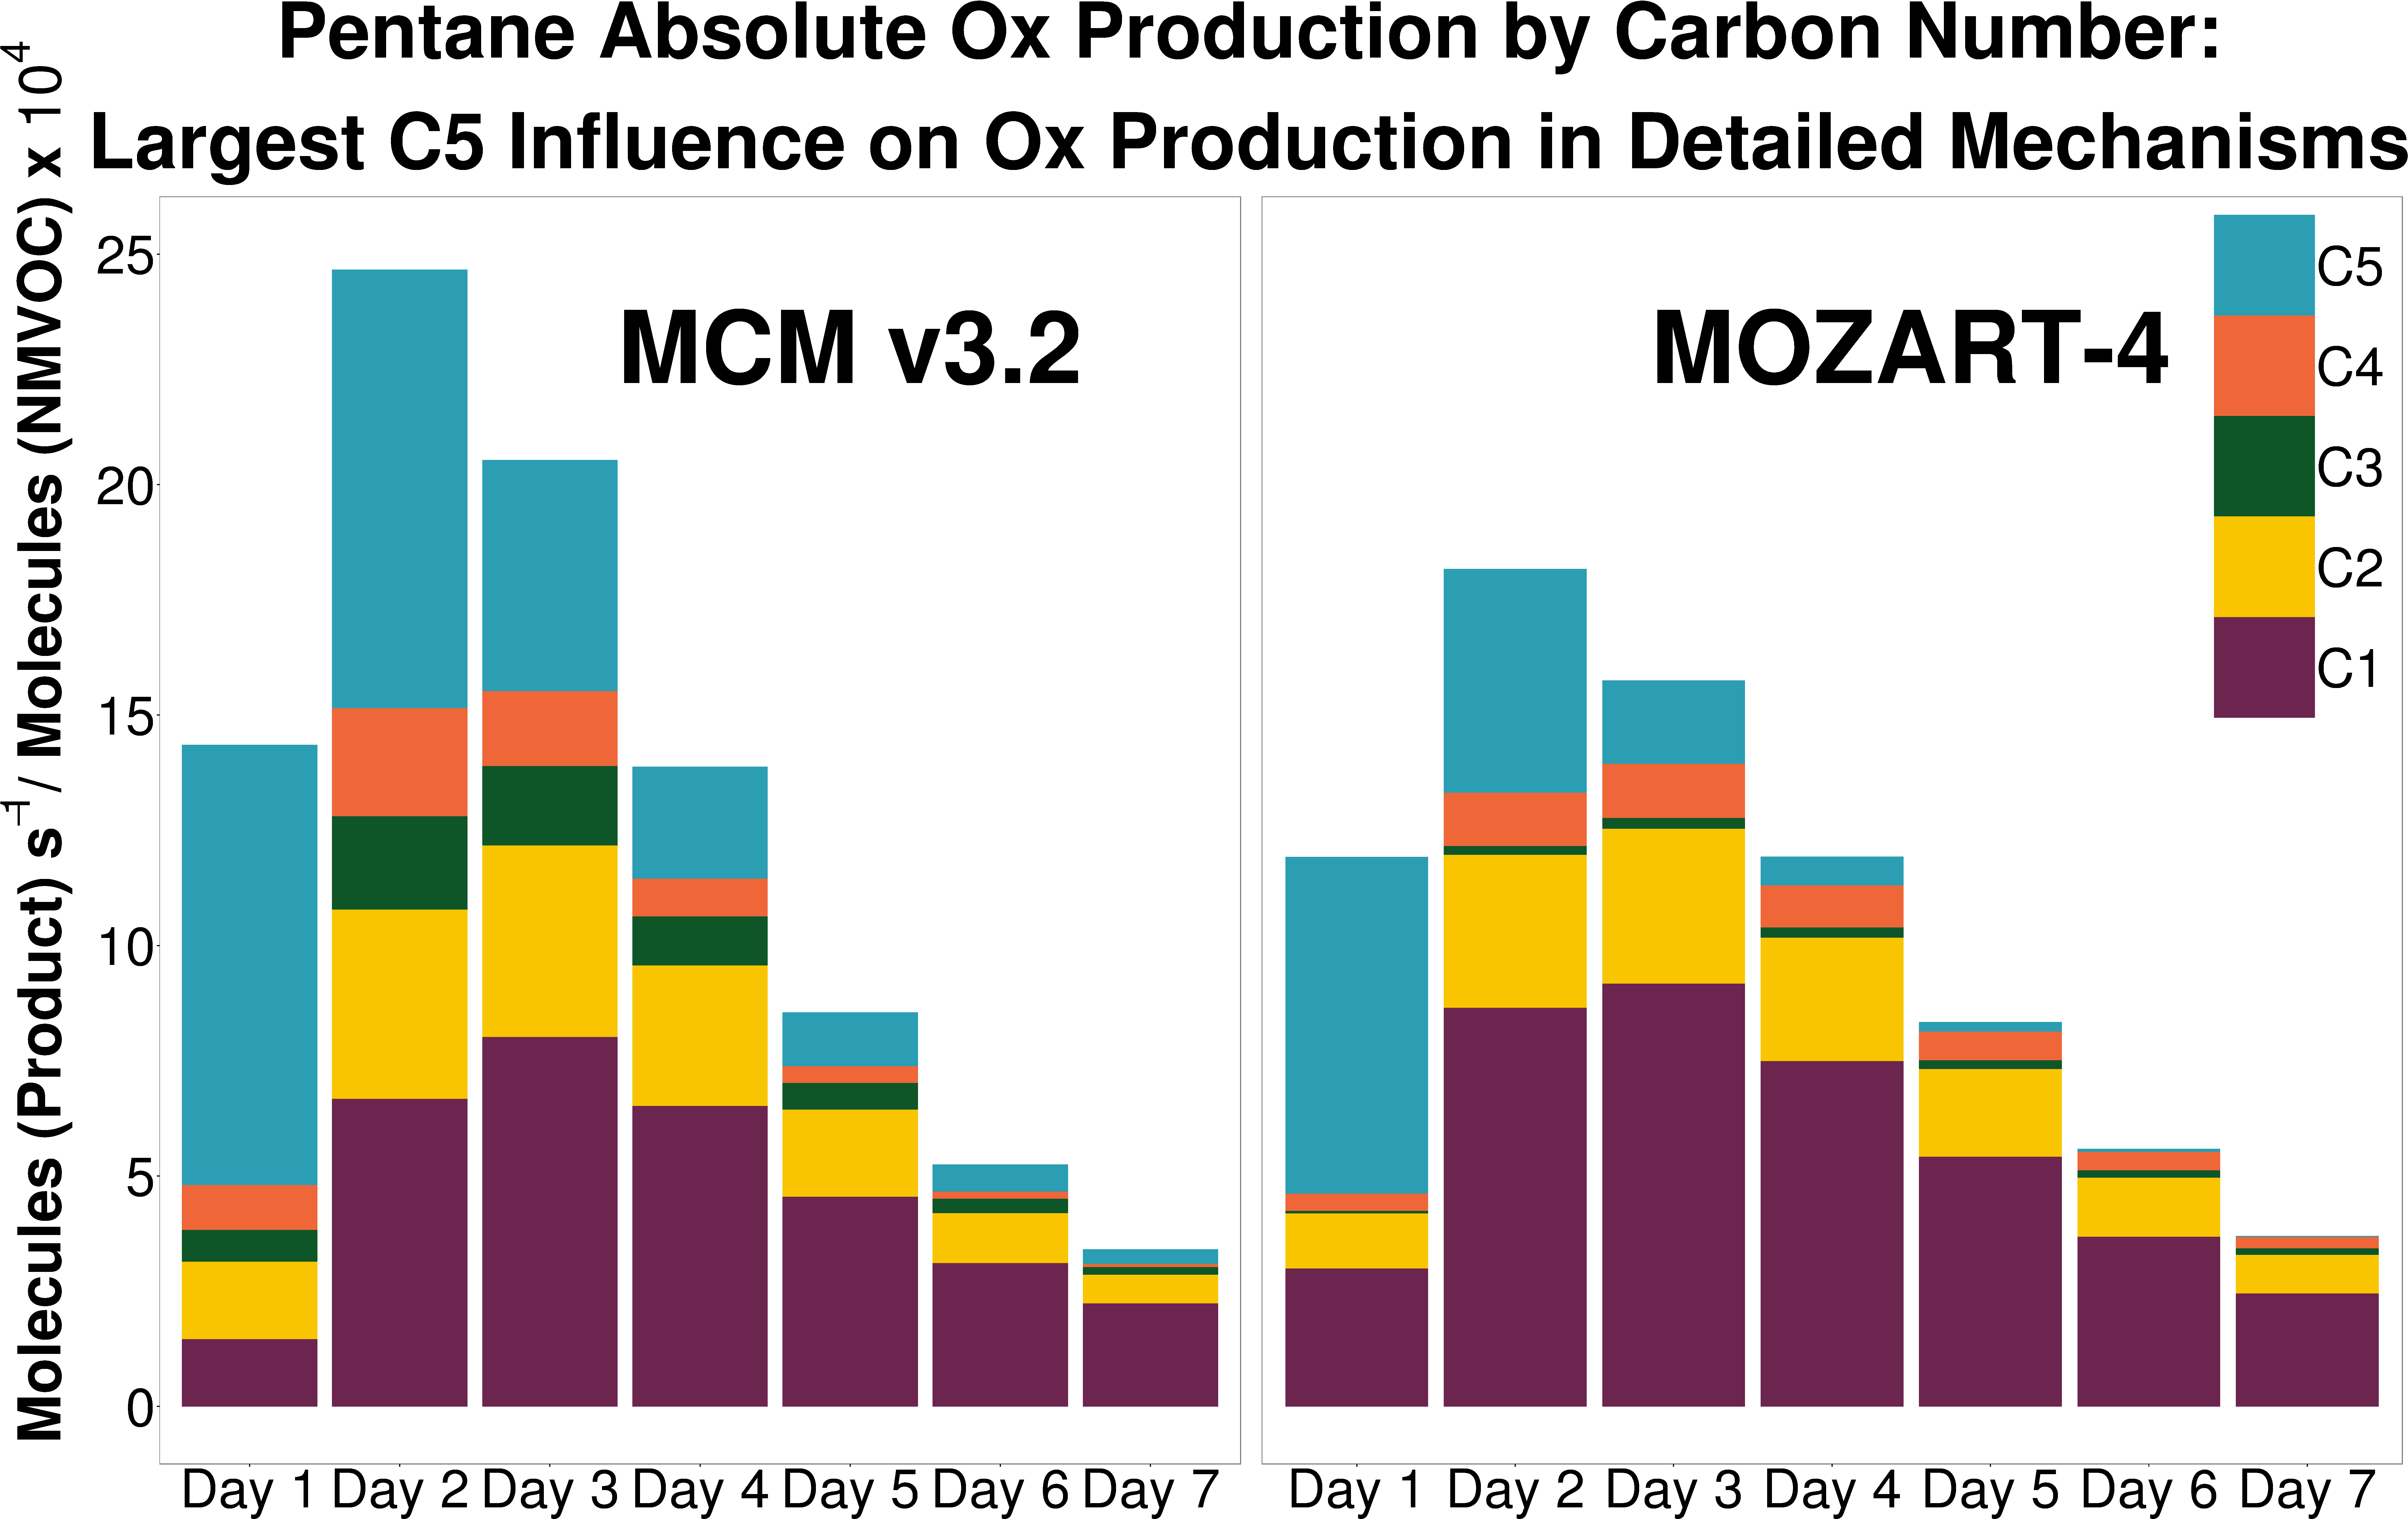
\includegraphics[scale=0.14]{img/pentane_carbon_breakdown}
                \end{center}
        \end{columns}
%        \tikzstyle{TOPP_box} = [draw=TitleBlue, rectangle, rounded corners, text width = 8.5cm, line width = 0.7mm]
%        \tikzstyle{aromatic_box} = [draw=TitleBlue, rectangle, rounded corners, text width = 12cm, line width = 0.7mm]
%        \tikzstyle{carbon_box} = [draw=TitleBlue, rectangle, rounded corners, text width = 13.5cm, line width = 0.7mm]
%        \begin{tikzpicture}[ultra thick, overlay]
%            \node (placement) {};
%            \node (dummy_TOPP_Tol) [above = 26cm of placement] {};
%            \node (TOPP_tol) [right = 46cm of dummy_TOPP_Tol] {};
%            \node (dummy_RACM) [above = 17cm of placement] {};
%            \node (RACM) [right = 55cm of dummy_RACM] {};
%            \path [-triangle 45, line width = 7mm, fill = TitleBlue, draw = TitleBlue] (TOPP_tol) edge node {} (RACM);%
%
%            \node (dummy_TOPP_Pen) [above = 26cm of placement] {};
%            \node (TOPP_Pen) [right = 28cm of dummy_TOPP_Pen] {};
%            \node (dummy_MOZART) [above = 17cm of placement] {};
%            \node (MOZART) [right = 19cm of dummy_MOZART] {};
%            \path [-triangle 45, line width = 7mm, fill = TitleBlue, draw = TitleBlue] (TOPP_Pen) edge node {} (MOZART);%
%
%        \end{tikzpicture}
    \end{block}
\end{GreyBox}
